% This example An LaTeX document showing how to use the l3proj class to
% write your report. Use pdflatex and bibtex to process the file, creating 
% a PDF file as output (there is no need to use dvips when using pdflatex).

% Modified 

\documentclass{l3proj}
\usepackage{datetime}
\usepackage{graphicx}

\begin{document}
\title{Algorithm Animator}
\author{Arthur Bigeard \\
		Alexander Ferguson \\
		Andrew Gibson \\
		Gediminas Leikus \\
		Liam Bell}
\usdate
\date{\today}
\maketitle
\begin{abstract}

Algorithm Animator - a teaching and learning tool for both students and teachers. A piece of software, which animates algorithms and produces a visual representation of how they work.

Our project - an API approach using Java and TimingFramework to develop the Algorithm Animator. Due to the fact that it is an API approach, the user of the software is required to know programming and Java, in particular, in order to use it. Animation of 3 common data structures - Arrays, Linked Lists and Binary Trees. Ability to export the animations to images or export Array animations to Flash.

\end{abstract}
\educationalconsent
\tableofcontents
%==============================================================================
\chapter{Introduction}
\label{intro}
Explaining complex algorithms or trying to understand them sometimes proves to be a difficult task even for experienced programmers, computer scientists and software engineers. Some of them are so huge and complicated, that it is hardly possible to remember and keep track of everything that is happening inside of it, therefore we often take a pen and a piece of paper and draw some sort of visualization of the algorithm and take notes in order to understand or explain them better. But what if you dont have a pen and/or a piece of paper? It often becomes messy as well and drawing, redrawing everything is rather time consuming. What if we are trying to develop a new and better algorithm and we want to see whether it is faster when compared to a conventional one? What if we want to visually see or show these differences?

The algorithm animator is an application dedicated to showing graphically the functionalities of a wide range of algorithms using the most common programming data structures. Our approach of the project is such that a novice developper can create his own custom animation to illustrate his algorithms. The data structures supported by our project include arrays, heaps and linked lists.

The project consists of an API providing object classes for each of those data structures and set of functions to instantiate an animation and add basic animation steps, such as object swaps and highlighting, which combined can provide a suitable graphic view of the running algorithm. Our project also provides solutions to run continuous or broken into step animations and backtracking of the steps taken. In order to emphasize the educational purpose of the application, it is also possible to display description sentences as each of the steps of the animation is running.

It is made very simple for the user to create powerful animations as he just needs to instantiate the animation object matching the data structure his algorithm uses and implant a small set of functions in his code to synchronize an animation with his running algorithm.

\section{Motivation}

Our project's main motivation is to provide developpers, lecturers an easy and comprehensive way to explain graphically educational algorithms or any of their own algorithms through the use of our API's animation functions, for the most common programming data structures. We know as students that learning from a pseudo-code or verbal explanations is often not the most efficient method and we wish to provide a simple to learn tool to increase developpers' teaching potential, and students' learning experience.

This project is suitable for use for novice JAVA developpers and should encourage its users to reflect on the most efficient ways to introduce graphically their algorithms to an audience and explain their purpose and functionning.

\section{Aims}
Our projects aim is to provide a tool, which would allow its users to easier visualize different, even unique or custom built algorithms and create animations out of them. We also want to make our system as general as possible in the sense of supporting a range of styles of algorithms, ability to export animations to different file formats, which could be easily viewed on different operating systems and devices.

The aim of this project is to create a complete, documented and well-built API to build animations in the most straight-forward way, while enabling the user to chose from a wide range of choice of animation and data structures. This includes the following tasks:
\begin{enumerate}
	\item Building graphically and animating:
	\begin{itemize}
		\item Arrays
		\item Heaps
		\item Linked Lists
	\end{itemize}
	\item Providing easily understandable functions to:
	\begin{itemize}
		\item Highlight elements
		\item Swap elements
		\item Display description messages
	\end{itemize}
	\item Creating an interface to control the displaying animation
	\item Enabling the end-user to export his animation in an executable format
\end{enumerate}

\section{Background}
Since part of Team Project 3 course curriculum is to work on a team project, we, as a group, chose this project from a list of provided project proposals as one of 5 projects we would like to work on and we were assigned to work on it. The project itself was proposed by our group project supervisor, Simon Gay. The main reason described in the project proposal what this software would mostly be used for was teaching purposes, therefore it seems academics are no exception and are also constantly looking for different ways to explain material for their students.

While our project does not build on any previous work and we are developing a solution from scratch, we have seen at least a few sorting algorithm animations during our ADS2 (Algorithms and Data Structures 2) course in second year (for example: \cite{website:Examples}). These animations were good examples and sources of ideas, which we are using in order to develop our software.

\section{Preliminaries}
While the report itself is hopefully going to be easy to read and understand to everyone, computing knowledge and experience (especially in Java programming language) is preferred, since our project involves developing an API and our end product will not be usable without having these skills. Also, parts of the report will also discuss Java (programming language) details or instructions on how to use a program written in Java and extend it to use our API to produce an animation.

\section{Outline}
The remainder of the report will cover:
\begin{itemize}
	\item Design - Domain model diagrams to describe the classes of the project's API and explanation of the reason why the TimingFramework graphics framework was chose over the other existing JAVA graphics frameworks.
	\item Implementation - this part will cover the tools and the methods use to code the API.
	\item API documentation - a list of the API classes including attributes and functions full description to help the end-user manipulating the API.
	\item Maintenance document - summarization of the delivered software, identifying all major deficiencies
	\item Summary log - abstract of the project log including all major contributions made by each individual
	student to the project
	\item Other documentation (for example: a user/reference manual or internal documentation)
\end{itemize}

%==============================================================================
\chapter{Design}
\label{design}

\section{Selection of a suitable graphics framework}


During the beginning of the project, several of my teammates and I were assigned to the research area where were to examine a suitable graphics framework that couldassist the team in building a solid animation API for our end users. During the research, we found there were several popular graphics frameworks for assisting with animation alongside Java applications, typically integrated through the use of compiled classes within a Java archive (.jar).

The range of frameworks proved problematic, given that it was most suitable to select a single framework to build with, otherwise there would be serious inconsistencies between developed applications (as they differ in their functionality) We established a simple set of fundamental criteria for selection as follows:
\begin{itemize}
	\item The framework should offer a fully functional API, of which can be accessed by our code in order to build animation.
	\item It should provide some degree of control, so that our own API can display dynamic movement and precision.
	\item It should be able to be in-cooperated into an integrated development environment (IDE) for group production during the implementation stage.
\end{itemize}

After careful research, we found three separate candidates for animation production with Java. In order to justify a suitable approach, each framework was considered separately to assess desirable characteristics and identify potential flaws. 

\underline{\textbf{Timing-Framework:}}

The Timing Framework was found on Java.net, a place for Java based libraries and extensions (\cite{website:TimingFramework}). It features controlled timing and ease of animation.

\textit{Advantages:}
\begin{itemize}
	\item The library is multi-threaded and concurrently safe. This prevents us from having to worry about complex synchronization issues between multiple application threads (as our animation software will utilise several threads for handling graphical changes independently)
	\item Uses less memory, putting a smaller load on systems with limited memory, allowing more applications to execute at once. 
	\item Offers an extensive API, giving us the ability of more control and functionality over our animations.
	\item Supportive of Swing and SWT development, for flexibility over a suitable distribution
	\item Its functionality can produce smooth, complex and controlled animation, useful for providing sufficient detail to our users in an orderly fashion.
	\item Can be in-cooperated easily into an existing Eclipse project (a solid Java development IDE, which all the team have good knowledge of)
\end{itemize}

\textit{Disadvantages:}
\begin{itemize}
	\item The API is detailed and complex in areas, which may invoke a steep learning curve.
	\item Swing examples documented are rather vague, and information given in a relevant PDF chapter is out dated.
\end{itemize}

\underline{\textbf{Java-FX:}}

Java-FX was found on the Oracle technology website (\cite{website:JavaFX}) it features UI based accelerated graphics. Its control is timeline based.

\textit{Advantages:}
\begin{itemize}
	\item Like the Timing-Framework, it also uses concurrently safe libraries.
	\item Potentially less complex to learn, given that Oracle have provided a more comprehensive set of documentation, including video tutorials.
\end{itemize}

\textit{Disadvantages:}
\begin{itemize}
	\item Newer libraries are not supported within Eclipse. This isn’t useful to us as a team as our preferred development environment is Eclipse. It is more suited to the Netbeans IDE, which we aren’t familiar with.
	\item It is more oriented towards web-based user interface development, typically within business. The goal of our application does not support this business approach, and focuses on the aspects of animation rather than an interactive interface with less emphasis on complex animation techniques.
\end{itemize}

\underline{\textbf{Trident:}}

Like the Timing-Framework, this was also found as part of a Java.net library development (\cite{website:Trident}) it’s focused entirely on timelines, namely duration and object changes across such durations represented by keyframes.

\textit{Advantages:}
\begin{itemize}
	\item Supports Swing and SWT development
	\item Allows multiple timeline events to be run and scheduled at any one time (multiple animations)
	\item Conceptually, it is straight forward and approachable; timelines represent the course of the animation and the keyframes the alterations to animation objects.
\end{itemize}

\textit{Disadvantages:}
\begin{itemize}
	\item Little documentation and not completely approachable as a result.
	\item It doesn’t seem to fully support concurrency as part of its API. To give an example, the code below taken from the documentation section on timelines demonstrates parallel timeline objects competing for shares properties(http://www.pushing-pixels.org/2009/06/25/trident-part-8-timeline-scenarios.html)
\end{itemize}

\begin{figure}
\begin{center}
\begin{verbatim}
        synchronized (this.circles) {
            circles.add(circle);
        }
        scenario.addScenarioActor(timeline);
    }
return scenario;
}...
public void paint(Graphics g) {
    synchronized (this.circles) {
        for (SingleExplosion circle : this.circles) {
            circle.paint(g);...
\end{verbatim}
\end{center}
\caption{Make a description up, Andrew}
\label{fig:frameworkExamples}
\end{figure}

In both examples \ref{fig:frameworkExamples} it can be seen that intrinsic locking is needed because of shared properties between objects. This adds a considerable degree of complexity to the framework, and would inevitably increase development time through the bugs and issues raised from concurrent access. For instance, if two objects were competing for shared animation data, and writing to it simultaneously, this would create unexpected behaviour. We would have to consider thread safe concepts alongside our own application complexity.

To conclude, we felt that the Timing-Framework offered the best and most approachable set of features. It provides multiple, dynamic animation techniques; with an emphasis on the animation itself as supposed to client designed web applications. It is also concurrent, which is hugely important as it draws a significant amount of complexity out the project. The animations we create will have their own threads delegated to tasks within the framework. The precision of control it offers is also an attractive trait, allowing us to build highly tweaked and well performing animations to our end users. 

Of course, the Timing-Framework is probably the most complex, but the positives most certainly outweigh the negative aspects. The analysis of these separate frameworks proved to be very useful in that sense, standing out as an important design choice that most likely would of saved us more development time in comparison to the other frameworks.

%==============================================================================

\section{Use cases}
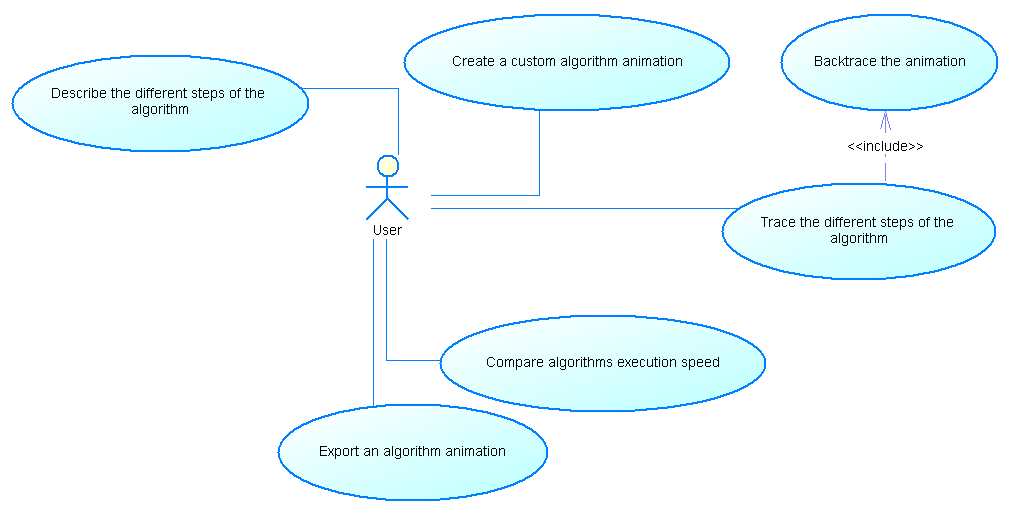
\includegraphics[width=115mm]{images/useCases.png}

Our use cases are meant to illustrate the main functionalities of our system. Using our API's, users will
be able to:
\begin{itemize}
\item Create custom algorithm animations on Linked Lists, Arrays and Heaps data structures
\item Display descriptions of the various steps of the animation as it processes
\item Navigate freely between the different steps of the animation backwards or forwards
\item Export animations in an executable format
\end{itemize}
\section{Components}
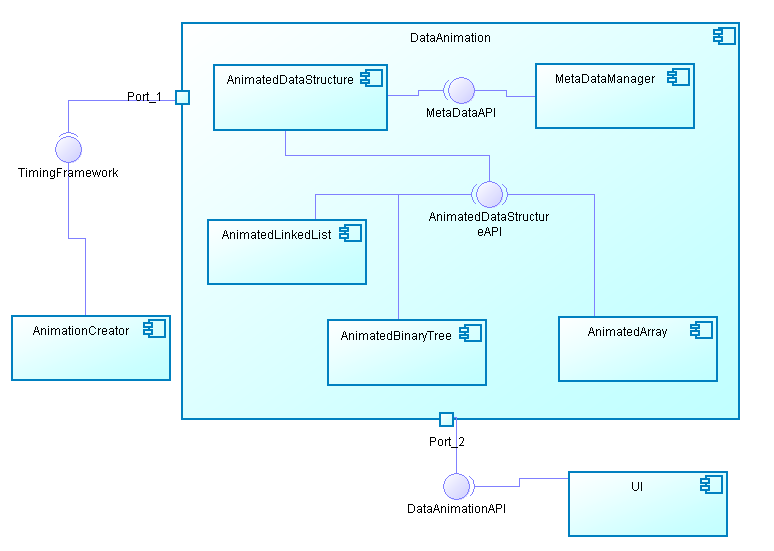
\includegraphics[width=115mm]{images/componentDiagram.png}

\section{Classes}
\subsection{AnimatedDataStructure Component}
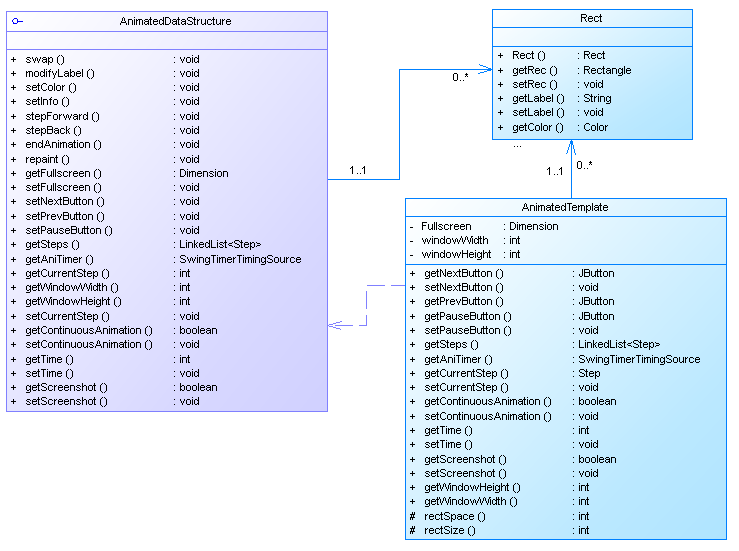
\includegraphics[width=115mm]{images/animatedDataStructureDiagram.png}

This diagram shows the component design of the system and their dependencies. The core of the system is the DataAnimation component,
which is relying on the Animation creating TimingFramework API, provided by a component labeled AnimationCreator.
The DataAnimation component is an aggregate of the components required to create a complete data animation, AnimatedDataStructure and MetaDataManager, and the data structure animation components
resulting from the use of the first two components. Our animations are called by the UI component to enable displaying them.
We can infer from this diagram the system architecture is a facade architecture, where the UI component is the facade component.

\subsection{AnimatedArray Component}
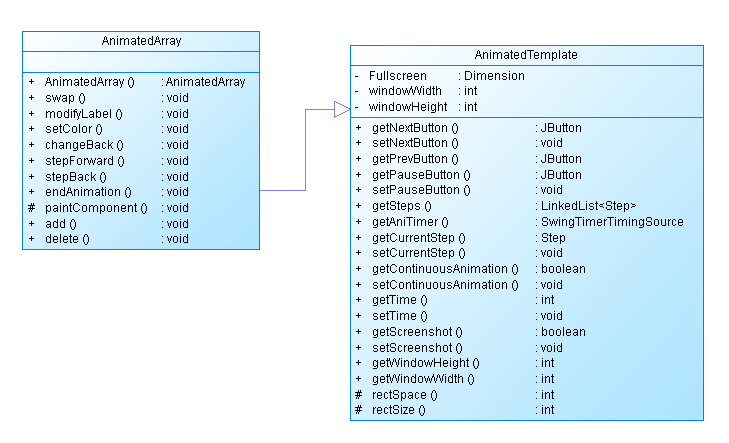
\includegraphics[width=115mm]{images/arrayDiagram.png}
\subsection{AnimatedLinkedList Component}

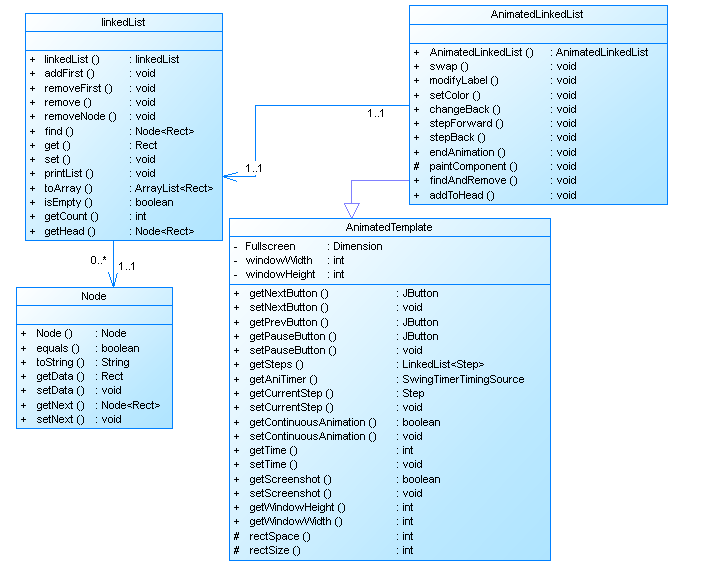
\includegraphics[width=115mm]{images/linkedListDiagram.png}
The AnimatedLinkedList data structure requires additional classes to store the Rect objects in a way that is coherent to the data structure.
The Rect's are stored in a custom linked list data structure implemented such that manipulating the data stored in the list will also update the display of
the linked list.
\subsection{AnimatedHeap Component}
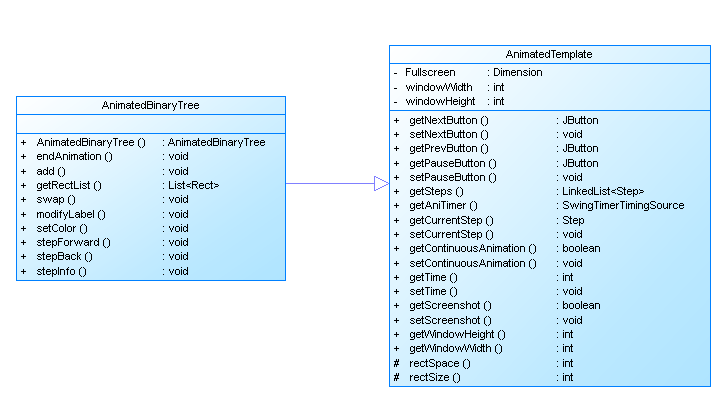
\includegraphics[width=115mm]{images/heapDiagram.png}
\subsection{MetaDataManager Component}
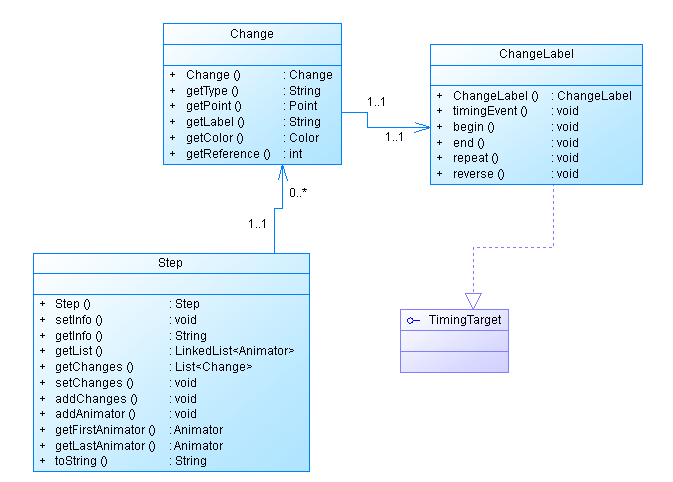
\includegraphics[width=115mm]{images/metaDataDiagram.png}
The MetaDataManager component provides a set of classes and functions meant to store the steps and step informations of the animations. The user manipulates
those data through the public animating calls made in the different data structures' classes.
\subsection{UI Component}
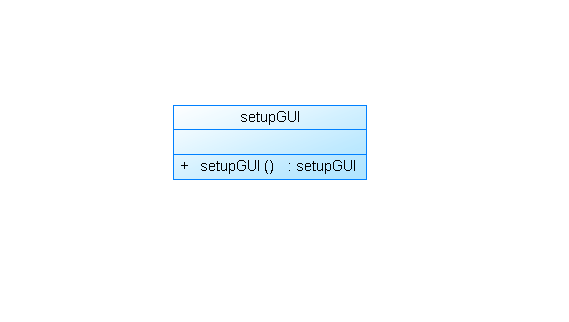
\includegraphics[width=115mm]{images/UIDiagram.png}
%==============================================================================
\chapter{Implementation}
\label{impl}

In this chapter, we describe how the implemented the system.

%------------------------------------------------------------------------------
\section{User Interface}

TODO

% - - - - - - - - - - - - - - - - - - - - - - - - - - - - - - - - - - - - - - -
\section{Problems Encountered}
\subsection{Arthur Bigeard}
Once our team got familiar with the TimingFramework, the application started rapidly growing and quickly our first animated algorithms were produced. 
On early stages of the animation display, we figured several features should be added to the display to increase the potential of our animations, features including:
\begin{itemize}
\item Labelling the steps of the animation
\item Navigating through steps from a list
\item Resizing dynamically the window to fit several animation demonstrations on a screen
\item Dynamically changing the speed of the animation using simple Speed Up/Speed Down JButtons
\end{itemize}

Introducing dynamic features to the animation constituted a challenge on several levels:
\begin{itemize}
\item performance-wise : the animation approach taken with the TimingFramework requires creating several objects per step; our approach of algorithm animation is such that animation are splitted
in a multitude of atomic steps and therefore consume a lot of memory
\item algorithm-wise : dynamic features require to look up and modify crucial data to the animation, where corruption of those data would lead to display inconsistencies or program termination
\item boundary-wise : our animations are limited by the animation framework we're using, the TimingFramework; we cannot implement what the TimingFramework cannot do
\end{itemize}

To illustrate better the challenges involved in implementing dynamic features, here is a list of data potentially subject to changes:
\begin{itemize}
\item Rect's and Rectangle's x/y coordinates and edge size
\item Step's Change Linked List 
\item Change's changed Object reference
\item Animation triggers, the Animator objects provided by the TimingFramework
\item setupGUI
\end{itemize}

Attempting to implement dynamic speed changing of the animation demonstrates very well the limits of the TimingFramework and our implementation:
\begin{figure}
\begin{center}
\begin{verbatim}
Step s = new Step(); // create a new step
// Create animation for showing information on what's happening
String information;
if (info == "") {
    information = "Swapping index " + a + " (" + rect_list.get(a).getLabel() + 
        ") " + " with index " + b + " (" + rect_list.get(b).getLabel() + ")"; // create the string
} else {
    information = info;
}
s.setInfo(information); // add it to the step
// Change information
s.addAnimator(new Animator.Builder().setDuration(1, TimeUnit.MILLISECONDS)
    .build(), s.getFirstAnimator()); // create an animator for this, which 
                                     //we could use to trigger this change
s.getLastAnimator().addTarget(new ChangeLabel(this, information, this));
// create a timing target to change the label when the animation starts	
// Create the Animators and PropertySetters (what should the animation change 
// the property from what to what) for swapping rects
s.addAnimator(new Animator.Builder().setDuration(time, TimeUnit.MILLISECONDS)
	.build(), s.getFirstAnimator()); // we want this Animator to start the same
// time the first Animator in the step does
s.getLastAnimator().addTarget(PropertySetter.getTarget(rect_list.get(a), 
	"currentY", rect_list.get(a).getRec().y, rect_list.get(a).getRec().y+rectSpace()));
s.addAnimator(new Animator.Builder().setDuration(time, TimeUnit.MILLISECONDS)
	.build(), nextBtn); // we want this Animator to start straight after the 
	// last Animator finishes. This is how it's done just now
s.getLastAnimator().addTarget(PropertySetter.getTarget(rect_list.get(a), "currentX", rect_list.get(a).getRec().x, rect_list.get(b).getRec().x)); 
s.addAnimator(new Animator.Builder().setDuration(time, TimeUnit.MILLISECONDS).build(), nextBtn);
s.getLastAnimator().addTarget(PropertySetter.getTarget(rect_list.get(a), "currentY", rect_list.get(a).getRec().y+rectSpace(), rect_list.get(a).getRec().y));		
//rect 2
s.addAnimator(new Animator.Builder().setDuration(time, TimeUnit.MILLISECONDS).build(), s.getFirstAnimator());															// we want this Animator to start the same time the first Animator in the step does
s.getLastAnimator().addTarget(PropertySetter.getTarget(rect_list.get(b), "currentY", rect_list.get(b).getRec().y, rect_list.get(b).getRec().y-rectSpace()));
s.addAnimator(new Animator.Builder().setDuration(time, TimeUnit.MILLISECONDS).build(), nextBtn);
s.getLastAnimator().addTarget(PropertySetter.getTarget(rect_list.get(b), "currentX", rect_list.get(b).getRec().x, rect_list.get(a).getRec().x));
s.addAnimator(new Animator.Builder().setDuration(time, TimeUnit.MILLISECONDS).build(), nextBtn);
s.getLastAnimator().addTarget(PropertySetter.getTarget(rect_list.get(b), "currentY", rect_list.get(b).getRec().y-rectSpace(), rect_list.get(b).getRec().y));
// Trigger for a continuous animation
s.addAnimator(new Animator.Builder().setDuration(1, TimeUnit.MILLISECONDS).build(), nextBtn);
s.getLastAnimator().addTarget(new ContinuousAnimation(currentStep+1, this));
// Log the changes in the Step
s.addChanges(new Change("swap", rect_list.get(a), rect_list.get(a).getRec().x, rect_list.get(a).getRec().y));
s.addChanges(new Change("swap", rect_list.get(b), rect_list.get(b).getRec().x, rect_list.get(b).getRec().y));
\end{verbatim}
\end{center}
\caption{Sample code from the AnimatedArray swap function}
\label{fig:swap}
\end{figure}

As you can see on this sample piece of code, the "core" of the animation, the Animator objects, are passed a static time value. We're keeping track of the Animators in a LinkedList stored in the corresponding step of the animation. A basic approach to the feature would be to simply browse every single Animator objects in our Step and modify the time value stored in the trigger using a simple speed ratio going from 0.25 to 4 for example. However, and this is where the TimingFramework failed to our expectations, once created, the Animator objects cannot be modified. Hence, it is not possible from this approach to implement dynamic speed change to the system.

At this stage, it was still possible to implement dynamic speed change to the animation. If we cannot modify our Animators, the logical next step to the solution is the re-create the Animators instead of modifying them. This alternate solution is extremely constraining:
\begin{itemize}
\item performance-wise : Re-creating the Animators involve 3 steps: browsing steps, destroying animators, re-creating them.
\item algorithm-wise : This solution requires heavy coding. While the first solution would only require to modify a time field, this solution requires to look up the type of Step we're currently modifying and the type of data structure we're animating in order to re-create the Animators properly
\item requirements-wise : Destroying the Animators object would obviously require us to restart the animation from the beginning; not only this is not the expected behaviour from a speed change button, this solution might also cause the application to hang due to the heavy object manipulation overhead
\end{itemize}

Due to too heavy constraints this solution was quickly dropped. With the current analysis of the implementation requirements for this feature, only one solution could reasonably be infered: static speed changing. As you've seen on (\ref{fig:swap}), we can specify the duration of the animation when creating the Animators; the solution adopted was that the user can specify his own time unit using the setTime call while creating an algorithm animation. 

Attempting to implement dynamic window resizing also showed the limits of our own implementation and especially of the Step management system. Although this solution was almost fully coded and working on a first and long attempt, we decided to give up on it for a cleaner, easier static resizing solution. Implementing this feature was very challenging regarding to the consistency of the Step data stored by the system. To get a better idea of the issues involved in dynamic resizing, here's a reminder of the potential data involved in resizing:
\begin{itemize}
\item Steps
\item Rects and Rectangles
\item Changes
\item setupGUI
\end{itemize}

Two implementations can be suggested for this feature; they both have their own perks and withdraws:
\begin{itemize}
\item Keeping a window width/height ratio relative to a fullscreen size from which the original x,y coordinates and size of the elements are calculated. The window width/height ratio would simply be used to adapt those x,y coordinates and element size. While this solution is very simple to code, it may lead to severe data inconsistency: using has a strong impact on the data precision, therefore, an expectableconsequence from this implementation is unaligned elements. However, it is important to notice that the performance overhead is neglectable.
\item Re-creating the data involved in window resizing. Practically, this solution requires a lot more coding. It is extremely unefficient for the same reasons explained on the dynamic animation speed changing. It would also require to restart the entire animation each time the window is resize.
\end{itemize}

The second solution can clearly be dropped due to its obvious disadvantages. In the process of coding, this is how we went about defining how we may implement dynamic window resizing.

The first solution was implemented; as expected, resizing resulted in unaligned elements. Usually, the scaling of the elements would be inconsistent from a range of 5 to 20 pixels.
We have considered the eventuality of adding a scaling function to align the elements after the resizing process and after each step. Again, this fix has huge disadvantages: scaling elements would be done
regardless to the position of the elements on the window, and multiple resizing may result in elements gradually moving up and down the window, and in the worst cases litterally working all their way up or down the window.
Why? Simply because scaling the elements would require to move them all up or down the window. Elements would no longer be centered. 
Again, performance-wise, this solution increases a lot the operations required to run steps on the animation.

Our team discussed the need for dynamic resizing, to either justify dropping this feature or keeping it and improving it so that it works perfectly.
We've decided to drop dynamic resizing for static resizing on the following assumptions:
\begin{itemize}
\item The user is unlikely to resize his window on a regular basis.
\item The user aims to demonstrate algorithms graphically. Where demonstration is involved, preparation is involved too. We can reasonably suppose that our end-users
will choose a fixed window size for their demonstration, if not fullscreen size, and keep the window to that size until the end of the animation. Therefore, determining the window
size statically will satisfy the need for users to determine a custom animation window size. 
\end{itemize}
\subsection{Alexander Ferguson}

Flash exporting: Compiling versus file reading.
	This particular problem is one that could not be fully solved, and caused a lot of frustration over the course of the creation of the Flash project. Initially working from a trial version of Flash Professional CS6, I was able to compile and run flash animations I had written. However when it came to using a command line compiler that could be called by the java program, I ran into a few problems. The main complication is that there are multiple different compilers, and the only free compiler I had found that seemed suitable to work on different operating systems - “Adobe FLEX” - was unable to compile .fla files - the file format of Flash Professional CS6. This left me confused for a while, until I found a free, open source IDE called FlashDevelop, which used a collection of actionscript 3 files, instead of compiling through the project. This seemed like the perfect solution, until I ran into another problem that again ground my workflow to a halt: The free FLEX compiler now worked, but was a subset of the professional version, missing the vitally important file IO systems. I then had the following choice between development platforms:
\begin{itemize}

\item Adobe Flash Professional CS6	

\textit{Advantages:}
\begin{itemize}
\item		This program is adobe’s high power flash flagship, and is a very good platform to learn to write flash applications on. Since it is the standard for creating flash applications, there are many tutorials and sites dedicated to helping create relevant code. The WYSIWYG editor generates code behind the scenes to help, which allows quicker implementation and more efficient debugging.
\end{itemize}

\textit{Disadvantages:}
\begin{itemize}
\item	To compile the files that are created, the user is required to have the official Adobe Flash program, version CS3 or greater. This requires that the user either spends a large amount of money for a license, or signs up for a free trial, both of which require downloading gigabytes of official Adobe software.
\item	Adobe flash professional has a strong focus on creating actual animations, using distinct, predefined frames of animation. This was a nuisance to manage the different frames of animation, and caused a lot of problems.
\end{itemize}

\item FlashDevelop
\textit{Advantages:}
\begin{itemize}
\item	The free software has the feeling of a real programming IDE. Using just a set of distinct actionscript class files, it is possible to create entire animations similarly to how it is done in java. By using a system of packages, include statements and method calls, you can link files together, which get compiled and grouped appropriately. There is no ‘hidden code’ in the animations, unlike Adobe Flash Professional, where it is possible to create objects in a frame, without being able to see the code for instantiating them. Although this increases time taken to implement the user interface, it is much more pleasant to maintain.
\end{itemize}

\textit{Disadvantages:}
\begin{itemize}
\item	The compiler used has only a subset of the functionality, lacking most importantly the ability to read or write from files before or after compilation. Without the ability to read the code from the user automatically, this tarnishes the very reasoning behind  the exporting component in the first place.
\end{itemize}

\textit{Solution:}
	At this point, an impasse occurs: either the program doesn’t compile, or it cannot receive any animation information. After getting frustrated, I decided that the only solution was to completely reinvent the component to an alternate form of exporting. Currently, the most suitable solution requires a small part of activity from the user that would have been unnecessary otherwise, where they now have a flash platform that can animate the objects from a user input, similar to the java program, from a string that is put into the pre-compiled .swf file.
	Before the java application has run once, The array objects are instantiated and the steps to be produced are recorded. There is a static String field in the AnimatedArray.java class that is appended to with the relevant information: first the array objects are instantiated, then the required swap and colour methods are called. At all of these stages, the code string is updated, and is then output to the file output.txt in the Exporting folder.
	The .swf file has two main classes: Steplist.as and Main.as. The Steplist class contains an object that holds the array values and operations, and contains a method to parse the input code from the user into a steplist object, which passes the information to main. The main class sets up the GUI and iterates over the operations. Because of inherent ability to resize flash animations, and have the objects automatically scale, The movement of the boxes is very simple: using a standard 50 pixels between the top corners of each box, it is possible to mimic the java program’s automatic box horizontal velocity by changing the x increment value. This is possible because of the functionality of actionscript timers: alongside the length of the timing window, is an additional variable to specify number of times to be invoked before finishing. This means that using a small timing window and a timer repeating count of 50, it is trivial to adjust the horizontal speed of the box. incrementing by 1 pixel allows a swap of adjacent components, and this increment value is simply increased to the value of the difference in array position.
	This solution completely erases all of the complexities in flash compiling, most notably getting it nullifies the project-affecting problems with releasing different software for each different operating system. The requirements for the user are also dramatically reduced, as the compiler alone requires 300+ megabytes of space for Adobe’s free flash compiler. This also reduces CPU usage for the java program. Assuming the .swf file would be compiled in the background once the steplist was finished, this could cause stuttering on older systems. 
\end{itemize}

\begin{itemize} 
\item Array positioning
 Once we had managed to successfully create an array of objects on the screen, I contributed with the basic display. Having created some early wireframes, I recreated them in java, with a simple formula to write 10 objects onto the screen to a window of fixed resolution. This was obviously suboptimal, since we required a way of displaying an array of any size, on any resolution. Looking at the different possibilities online, I found that the simplest way to be able to use the entire resolution of the screen was using a method I came across called getScreenSize() using java’s own java.awt.Toolkit. Using the screen width found, along with the number of array objects to be displayed, there was enough independent variables in the equation to determine the position and size attributes of the objects on screen. The size of the boxes, the size of the space between boxes and positioning of the array was determined by a short algorithm using the found screen size, number of objects and a fixed minimum spacing between objects of one pixel. This allows the user to enter an array of over 100 values, much more than would be required or useful. At this size, the text label on each object becomes unreadable on normal resolution screens, but is still fully functional as an animated array. 

\item Screenshot system for exporting as slides.
 One of the early permutations for exporting was to use a call to an external toolkit to save screen images that could be used in a slide show. Andrew had already started to add the functionality, but by separating it into its own class and using the java.awt.Robot toolkit, it was possible to create a new screenshot upon completion of every swap and colour change, store it in a folder and name it accordingly so that it can be iterated over and used as a slideshow if required. Andrew attempted to use the frame of the window to be the borders of the screenshot, but ran into problems with different screen sizes. To get around this, we reused the default toolkit that we had previously use to get the user’s screen resolution. This allowed us to capture the screen size of any system that the user is running the program on. Then, using another toolkit called Robot, we could call a method that would capture an image of the specified size:
robot.createScreenCapture(Rectangle screen) . This had the downside of also capturing the edges of the screen, and the top bar of the java window, but we agreed that since it was not going to be our long term solution to exporting animations, we could cope with the extra pixels.

\item Flash Exporting 
 Once the main program was nearing completion, I volunteered to take responsibility for the Flash exportation. None of us had any real experience with creating Flash files, except Andrew who was still in the process of implementing linked lists. Although the language had been largely modified in the update from Actionscript 2.0 to Actionscript 3.0 since he last used it, he gave valuable help with learning the language.
The initial plan was to incorporate an external compiler to trigger once the main java animation was created, compiling a .swf of the most recent animation that can be saved and reused as the java animation being displayed to the user. This plan was unanimously decided to be beyond the scope of the project, increasing the total complexity and requiring a lot of system redesign. The plan was scrapped when we discovered the difficulties in getting the data sharing between the programs, and automatic compilation of the .swf consistent between operating systems.
 The final version of the Exporting component is as follows. The java application, upon completing its steplist, concurrently creates a code string then outputs it to a file. The code string is a descriptor of the array created, and the operations performed on them. This string has a specific syntax that I created to be easy to parse in actionscript, and is described as follows:
“[instantiated values of AnimatedArray object]:[-operation]*”
Operations are either a swap - two index arguments - or a colour change: an index value followed by three arguments for the object’s desired colour’s red, green and blue channels. For example, the following code creates an array of five objects, swaps the objects at index 1 and 3, then changes the colour of the middle element to Black: 
0,1,2,3,4:-1,3-2,0,0,0

The final state of the animation is shown below.

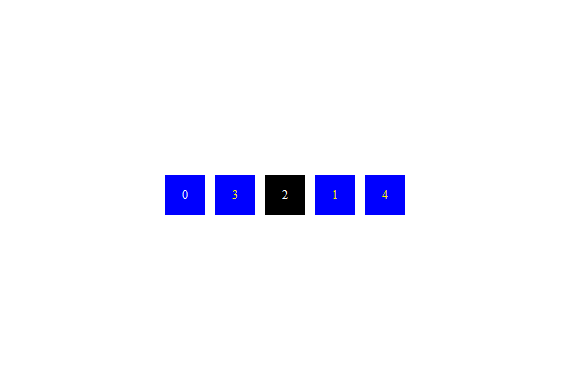
\includegraphics[width=115mm]{images/flash1.png}


Although it was an unfamiliar language to us, it became apparent that it would be possible to create an identical system, given enough time. The flash exporting component however was never intended to repeat the algorithmic functionality of the main program, so to prevent duplicating code and to save time, we decided to only implement a subset of the system. There is no functionality for a user to create their own algorithms in its current version, and there is only the ability to visualise AnimatedArray structures. Flash has its own built in resizing of the animation frame, but cannot scale as well as the java version of the implementation. Being a .swf file however, it comes with the added benefits of being able to be run on all current web browsers, embedded it in slide shows and applications, and can be referenced in html to be used in web pages.
\end{itemize}

<<<<<<< HEAD
=======
\subsection{Andrew Gibson}
\subsubsection{The selection of a suitable animation framework}
\label{frameworkSelection}

During the beginning of the project, several of my teammates and I were assigned to the research area where were to examine a suitable graphics framework that could assist the team in building a solid animation API for our end users. During the research, we found there were several popular graphics frameworks for assisting with animation alongside Java applications, typically integrated through the use of compiled classes within a Java archive (.jar).

The range of frameworks proved problematic, given that it was most suitable to select a single framework to build with, otherwise there would be serious inconsistencies between developed applications (as they differ in their functionality) We established a simple set of fundamental criteria for selection as follows:
\begin{itemize}
	\item The framework should offer a fully functional API, of which can be accessed by our code in order to build animation.
	\item It should provide some degree of control, so that our own API can display dynamic movement and precision.
	\item It should be able to be in-cooperated into an integrated development environment (IDE) for group production during the implementation stage.
\end{itemize}

After careful research, we found three separate candidates for animation production with Java. In order to justify a suitable approach, each framework was considered separately to assess desirable characteristics and identify potential flaws. 

\underline{\textbf{Timing-Framework:}}

The Timing Framework was found on Java.net, a place for Java based libraries and extensions (\cite{website:TimingFramework}). It features controlled timing and ease of animation.

\textit{Advantages:}
\begin{itemize}
	\item The library is multi-threaded and concurrently safe. This prevents us from having to worry about complex synchronization issues between multiple application threads (as our animation software will utilise several threads for handling graphical changes independently)
	\item Uses less memory, putting a smaller load on systems with limited memory, allowing more applications to execute at once. 
	\item Offers an extensive API, giving us the ability of more control and functionality over our animations.
	\item Supportive of Swing and SWT development, for flexibility over a suitable distribution
	\item Its functionality can produce smooth, complex and controlled animation, useful for providing sufficient detail to our users in an orderly fashion.
	\item Can be in-cooperated easily into an existing Eclipse project (a solid Java development IDE, which all the team have good knowledge of)
\end{itemize}

\textit{Disadvantages:}
\begin{itemize}
	\item The API is detailed and complex in areas, which may invoke a steep learning curve.
	\item Swing examples documented are rather vague, and information given in a relevant PDF chapter is out dated.
\end{itemize}

\underline{\textbf{Java-FX:}}

Java-FX was found on the Oracle technology website (\cite{website:JavaFX}) it features UI based accelerated graphics. Its control is timeline based.

\textit{Advantages:}
\begin{itemize}
	\item Like the Timing-Framework, it also uses concurrently safe libraries.
	\item Potentially less complex to learn, given that Oracle have provided a more comprehensive set of documentation, including video tutorials.
\end{itemize}

\textit{Disadvantages:}
\begin{itemize}
	\item Newer libraries are not supported within Eclipse. This isn’t useful to us as a team as our preferred development environment is Eclipse. It is more suited to the Netbeans IDE, which we aren’t familiar with.
	\item It is more oriented towards web-based user interface development, typically within business. The goal of our application does not support this business approach, and focuses on the aspects of animation rather than an interactive interface with less emphasis on complex animation techniques.
\end{itemize}

\underline{\textbf{Trident:}}

Like the Timing-Framework, this was also found as part of a Java.net library development (\cite{website:Trident}) it’s focused entirely on timelines, namely duration and object changes across such durations represented by keyframes.

\textit{Advantages:}
\begin{itemize}
	\item Supports Swing and SWT development
	\item Allows multiple timeline events to be run and scheduled at any one time (multiple animations)
	\item Conceptually, it is straight forward and approachable; timelines represent the course of the animation and the keyframes the alterations to animation objects.
\end{itemize}

\textit{Disadvantages:}
\begin{itemize}
	\item Little documentation and not completely approachable as a result.
	\item It doesn’t seem to fully support concurrency as part of its API. To give an example, the code below taken from the documentation section on timelines demonstrates parallel timeline objects competing for shares properties(http://www.pushing-pixels.org/2009/06/25/trident-part-8-timeline-scenarios.html)
\end{itemize}

\begin{figure}
\begin{center}
\begin{verbatim}
        synchronized (this.circles) {
            circles.add(circle);
        }
        scenario.addScenarioActor(timeline);
    }
return scenario;
}...
public void paint(Graphics g) {
    synchronized (this.circles) {
        for (SingleExplosion circle : this.circles) {
            circle.paint(g);...
\end{verbatim}
\end{center}
\caption{Make a description up, Andrew}
\label{fig:frameworkExamples}
\end{figure}

In both examples \ref{fig:frameworkExamples} it can be seen that intrinsic locking is needed because of shared properties between objects. This adds a considerable degree of complexity to the framework, and would inevitably increase development time through the bugs and issues raised from concurrent access. For instance, if two objects were competing for shared animation data, and writing to it simultaneously, this would create unexpected behaviour. We would have to consider thread safe concepts alongside our own application complexity.

To conclude, we felt that the Timing-Framework offered the best and most approachable set of features. It provides multiple, dynamic animation techniques; with an emphasis on the animation itself as supposed to client designed web applications. It is also concurrent, which is hugely important as it draws a significant amount of complexity out the project. The animations we create will have their own threads delegated to tasks within the framework. The precision of control it offers is also an attractive trait, allowing us to build highly tweaked and well performing animations to our end users. 

Of course, the Timing-Framework is probably the most complex, but the positives most certainly outweigh the negative aspects. The analysis of these separate frameworks proved to be very useful in that sense, standing out as an important design choice that most likely would of saved us more development time in comparison to the other frameworks.
>>>>>>> 3c1387f48dfd089b6831db20c1c1e08ffba7d0b1

\subsubsection{Development of Animated Linked Lists}

For part of the project involved linked lists - developed with Gediminas’s existing system on the back of the framework. The trigger design that Gediminas created for scheduling animations in a step based fashion was used for this, so that the user can step through each part individually. To begin with, a linked list class with generic nodes was created, which would eventually function as objects associated with animations. The linked list was represented as an array of these generic node objects. There were several problems encountered when attempting to in-cooperate the step-based animation classes into my own code. It became apparent that some of the step-based algorithms involved with the successfully built Animated-Array class didn’t directly translate to the Animated-Linked-List structure. A step in this sense is represented as a series of animations, as noted before.

The intention of the Animated-Linked-List class was to offer specific algorithmic operations associated with linked list data structures (as these were only applicable). One of the main issues encountered was attempting to implement a suitable algorithm to locate and remove all instances of a specific node in the list. Addressing the step-based approach for this algorithm, it was required that the deletion of each found copy of the node was represented as a step. Initially, an algorithm was developed to directly remove any found occurrences from a list of objects.

\begin{figure}
\begin{center}
\begin{verbatim}
while(node.getNext() != null && !(node.getData().getLabel().equals(i))){
    prev = node; //pointer to previous node
    setColor(count,Color.RED,"Changing color to red");
    setColor(count,Color.BLUE,"Changing color to blue");
    node = node.getNext();
    count++;
}
anim.setColor(count,Color.GREEN,"Changing color to green");
anim.setColor(count,Color.WHITE,"Changing color to white");
(**) prev.setNext(node.getNext());   //joins the pointer for the prev element after the to be deleted node
(**) rect_list.removeNode(node); //removes this node
\end{verbatim}
\end{center}
\caption{Make a description up, Andrew}
\label{fig:linkedListsExample}
\end{figure}

This proved to be problematic. Once executed, the animation would display the deleted node to the user, before they have even stepped through the animation and eventually reached the deletion of the found node. The early implementation of the problem highlights this issue (\ref{fig:linkedListsExample}).

This section of code (\ref{fig:linkedListsExample}) represents a linear scan across each of the list’s pointers, until the required node is found. When a node is found, it is highlighted, and subsequently deleted. The last two lines indicated by (**) in this piece of code highlight the issue. Although the overall method for locating and removing a node is represented as a step, the changes made directly to the linked list object (represented here as rectlist) are not stored in any structures that allow the user to step through. Hence, when the application is executed, these adjustments are already displayed to the user. 

To solve this issue, we proposed a solution that represented the main deletion operation as a single change within the method. In this way, the method would still be represented as a step (with its collection of animations) but the change class would allow us to log the deletion, so that we can obtain it and handle the deletion where necessary.

\begin{figure}
\begin{center}
\begin{verbatim}
if (steps.get(currentStep).getChanges().get(0).getType() == "deleteNode") {
    Node<Rect> p = steps.get(currentStep).getChanges().get(0).getNodeReference();
    rect_list.removeNode(p, p.getNext(),rectSpace(rectSize()));
} 
\end{verbatim}
\end{center}
\caption{Make a description up, Andrew}
\label{fig:linkedListsDeletion}
\end{figure}

It simply involved omitting the problematic lines above (**), and substituting a change to represent a deletion, with a reference to the object that is requested to be deleted. Once these changes were logged, the stepForward method allowed us to catch the corresponding change log at the appropriate time during the animation. A string comparison is done on the change log list and once it is found, the operations are then done on the linked list in order to display the deletion to the user. The code below shows part of the stepForward method. The change “deleteNode” is added after a node is requested to be deleted in the removal method, and a separate method in the linked list class handles the deletion of the specific node with reference ‘p’. The string “deleteNode” is caught at the appropriate time, given that the ordering of the steps is consistent in the application (\ref{fig:linkedListsDeletion}).

Another issue encountered involved the sequencing of steps, where the deletion of the node was not shown when cycling through steps. A solution was generated for this rather complex problem, which involved maintaining the correct ordering in the animation:

Our application calls methods when executed, and generates a list of steps (each of which has their own set of animations). To ensure the correct ordering of steps, a counter is incremented whenever a step is created in the program, so that when the user is stepping through, the correct step is executed next in the list sequence. The step is created when a method is called (removal in this case), and is to be represented as an animated sequence of some form. A step is then added to the list of steps once the method returns.

Originally when called the removal method would increment this counter, change the colour of the current node to indicate it is to be deleted, and finally change its colour to match the background to indicate deletion. Other methods were called inside of the removal method where they themselves incremented this counter. This caused inconsistencies in the ordering.

The step list is designed to execute the element ahead the counter’s value in the list, by triggering it and causing it to run the desired animation. 
In the current system, here is how the execution would have affected the ordering:

Say to begin with this counter was currently equal to 6 (assume the counter has the value 6). Assume the step list is ‘S’ = […6] initially, and has 5 step elements prior to it. The method findAndRemove(..) being the method involved in removing all occurrences of an item in the list.
Assume the colour changing method is called setColor(..), where it changes the colour of the node passed as an argument.

\begin{itemize}
\item The removal method is called, a step is instantiated
\item the counter is incremented (counter = 7)
\item setColor(..) is called to change the colour initially, this creates another step and increments the counter (counter = 8)
\item Once setColor(..) returns 8 is added to the list (S = […6,8]) 
\item setColor(..) is called a second time, returns and adds, and the list is now (S = […6,8,9], counter = 10) 
\item Finally findAndRemove(..) is returned to, and is finally added to the step list prior to exiting its own method. (S = […6,8,9,7])
\item When the user requests to step through the animation and requests the last element 7, the application will attempt to trigger the 10th element, as its relative position is 9. This will cause the application to crash as it attempts to access an out of bounds array index. The other steps will be inconsistent in their operation as well.
\end{itemize}


The desired ordering is therefore S  = [...6,7,8,9]. To achieve this, the counter was incremented after the method calls for both the colour adjustments. To explain:
\begin{itemize}
\item The removal method findAndRemove(..) is called, a step is instantiated
\item Both setcolor(..) methods are called, they both increment independently and append to the list of steps ( S = […6,7,8]
\item Once they return, the counter is incremented in findAndRemove(..) and the 9th step is added ( S = […6,7,8,9])
\end{itemize}

When the user steps through, step 6 will trigger the 7th element in the step list, the 8th will trigger the 9th animation and so on. Hence, the ordering is maintained and the application performs successfully.

<<<<<<< HEAD


\subsection{Gediminas Leikus}
\label{Gediminas:PE}
\subsubsection{Separating animations into steps and making continuous animations}
=======
\subsection{Separating animations into steps and making continuous animations}
\label{PE:steps}
>>>>>>> 3c1387f48dfd089b6831db20c1c1e08ffba7d0b1

The group decided to use Java for our project, because we were all familiar with it and because it was the language our client suggested us to use. For the reasons stated in this document \ref{frameworkSelection}, we decided to choose the Timing Framework \cite{website:TimingFramework}.

Our first Timing Framework animation example (\ref{fig:firstPrototype}) had multiple rectangles created from an array moving back and forth, had buttons allowing us to stop the animation, resume it or delete one of the rectangles.

\begin{figure}
\begin{center}
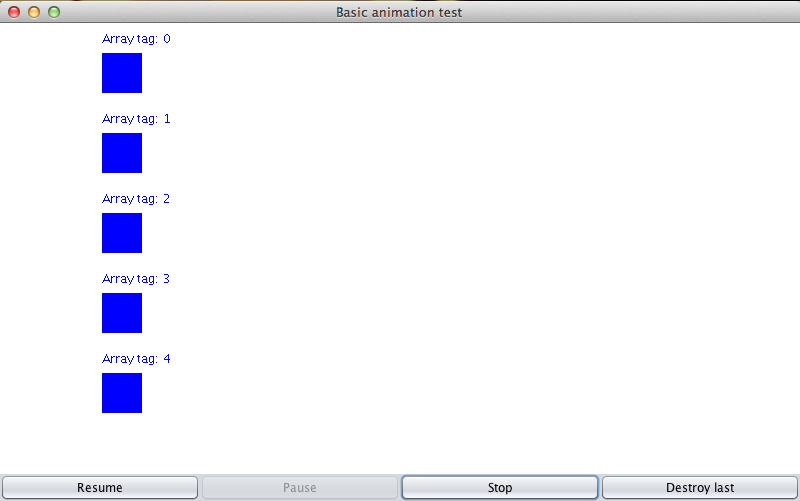
\includegraphics[width=\textwidth]{images/firstPrototype.png}
\end{center}
\caption{The first demonstration, produced by Andrew}
\label{fig:firstPrototype}
\end{figure}

While this was a good initial step, we did not have any obvious way to implement Steps, in a sense where multiple Animations could be assigned to one step and we could navigate through these steps back and forth. Therefore we started looking into it.

\begin{figure}
\begin{center}
\begin{verbatim}
public void timingEvent(Animator source, double fraction){
    boolean done = false;
    if(anArr.getToDo().size() > 0){
        Step[] steps = new Step[anArr.getToDo().peek().length];
        System.arraycopy(anArr.getToDo().peek(), 0, steps, 0, steps.length);

        for(int i = 0; i < steps.length; i++){                    
            Rectangle rect = rect_list[steps[i].getIndex()].getRec();
            double x = steps[i].getX();
            double y = steps[i].getY();
            double stepX = rect.getX();
            double stepY = rect.getY();
            if(y != stepY){
                if(Math.abs(x - stepX) < 50){
                    if(y > stepY){
                        rect_list[steps[i].getIndex()].getRec().x += 1;
                    }
                    else{
                        rect_list[steps[i].getIndex()].getRec().x -= 1;
                    }
                }
                else{
                    if(y > stepY){
                        rect_list[steps[i].getIndex()].getRec().y += 1;
                    }
                    else{
                        rect_list[steps[i].getIndex()].getRec().y -= 1;
                    }
                }
            }
            else{
                if(x > stepX){
                    rect_list[steps[i].getIndex()].getRec().x += 1;
                }
                else{
                    rect_list[steps[i].getIndex()].getRec().x -= 1;
                }
            }
            if(y == stepY && x == stepX){
                done = true;
                anArr.getToDo().poll();
                anArr.getDone().add(steps);
                break;
            }
        }
        repaint();              

    }
\end{verbatim}
\end{center}
\caption{Arthur example code making an animated change in coordinates}
\label{fig:arthurPrototype}
\end{figure}

Our first prototype implementation seemed: 
\begin{itemize}
	\item too complex (a swap of 2 rectangles was over 50 lines long \ref{fig:arthurPrototype})
	\item impractical to use (it didn’t have any way to step back and forth through the animation) 
	\item it had a performance overhead (all Animator objects were running continuously, until the whole animation was stopped)
\end{itemize}
It had a few good points though: 
\begin{itemize}
	\item it was done on a low level (so the how-to part was obvious if you understood the code) 
	\item it was not storing too much information (thus it did not really have a memory overhead). 
\end{itemize}
But this was not what we wanted – the most important thing for us was the stepping back and forth functionality.  Therefore we looked into it again.

During our research of the Timing Framework we found out that we could add triggers, which would start an animation, to a button or to another animation, which would start another animation when it stops or starts running \cite{website:TimingFrameworkDemo}. Thus, triggers seemed like a great tool for linking multiple animations into one Step, linking steps and making a continuous animation.

\begin{figure}
\begin{center}
\begin{verbatim}
s.addAnimator(new Animator.Builder().setDuration(time, TimeUnit.MILLISECONDS)
	.build(), nextBtn);

s.getLastAnimator().addTarget(PropertySetter.getTarget(rect_list.get(b), 
	"currentX", rect_list.get(b).getRec().x, rect_list.get(a).getRec().x));}
\end{verbatim}
\end{center}
\caption{My example code making an animated change in coordinates}
\label{fig:gPrototype}
\end{figure}

We still wanted to find a way to make a change of a rectangle (or any other object) property easy to manage. Looking through the Demos we also found that we could use Targets and PropertySetters to do this in just a few lines of code \ref{fig:gPrototype}, which seemed great. But it only allowed us to change a property, which was numerical (like coordinates or colors) – it didn’t allow us to change all the properties of the object, like the labels of rectangles. To solve this issue, we researched further and found that we can create a class, which would implement a TimingTarget interface and its begin(), end(), repeat() and reverse() methods. Therefore, to solve the issue of for example changing the labels of rectangles, we created a new class called ChangeLabel, which implemented a TimingTarget interface, its begin(), end(), repeat() and reverse() methods, and added a change of String variable just inside its begin method. This approach seemed great, because:
\begin{itemize}
	\item we can change any property of an object or do pretty much anything when that TimingTarget is called
	\item it is attached to each Animator object, so we do not have to worry about storing the TimingTargets anywhere
	\item it is efficient performance wise, because these TimingTargets are only executed, when the Animator object is
	\item it is easy to use, implement and understand
\end{itemize}

Therefore, the end result of our second prototype was:
\begin{itemize}
	\item a list of steps
	\item an array of rectangles and their coordinates at each step
	\item an ability to either step back and forth through the animation by using buttons or see a continuous animation (and it was either that or that)
\end{itemize}

After looking through both of our prototypes, we decided to merge the good parts of each: we kept most of second prototype, but reduced the amount of data stored for each Step, in particular, we made it so it would only store the details of the changed object before the change, rather than the details of all the objects.

The only issue left then, was the ability to have both step-by-step and continuous animations and allow the user to switch between them at any point of time, but this was not a big issue, since we just used a similar approach we used with ChangeLabel class:
\begin{enumerate}
	\item We created a new class, called ContinuousAnimation, which was also implementing the TimingTarget interface
	\item introduced a boolean variable called continuousAnimation, which was keeping record of whether the animation was in step-by-step or continuous mode
	\item made it so that the begin method in ContinuousAnimation would execute different actions according to the boolean continuousAnimation variable value:
	\begin{itemize}
		\item If true, Trigger the next Step
		\item If false, do nothing
	\end{itemize}
\end{enumerate}

\subsection{Refactoring}
\label{PE:refactoring}

Our first common implementation that we were using for development was coupled too much with AnimatedArray data structure (which was the first data structure we did) and was not flexible at all. This became obvious, when we started implementing our AnimatedLinkedList. When we wanted to make our API to animate an AnimatedLinkedList instead of AnimatedArray, we had to change multiple classes, including Rect, ContinuousAnimation and ChangeLabel \ref{fig:coupling}. This was due to no polymorphism in our implementation.

\begin{figure}
\begin{center}
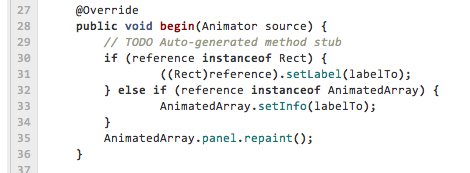
\includegraphics[width=\textwidth]{images/coupling.png}
\end{center}
\caption{ChangeLabel begin method dependency on AnimatedArray}
\label{fig:coupling}
\end{figure}

After doing our Professional Software Development 3 (PSD3) D7 deliverable (which was implementation of an Internship Management System we were designing the entire first semester), we have learned how to structure software better and how we can split code into components in Java. Therefore it was time for refactoring.

One of the first things we did was create a separate package for each data structure. This lead to 4 additional packages being created:
\begin{itemize} 
	\item AnimatedArray
	\item AnimatedBinaryTree
	\item AnimatedDataStructure
	\item AnimatedLinkedList
\end{itemize}
Each package is supposed to keep classes relevant only to its data structure, apart from AnimatedDataStructure package, which keeps classes that are relevant to all data structures.

We also completely separated the GUI from the rest of the code and created a class called setupGUI.

\begin{figure}
\begin{center}
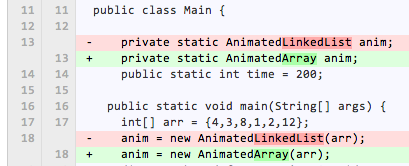
\includegraphics[width=\textwidth]{images/changeStructure.png}
\end{center}
\caption{Changing animation to animate a different data structure}
\label{fig:changeStructure}
\end{figure}

The next thing we did was create a public interface AnimatedDataStructure, which is how we solved the issue we mentioned in the first paragraph. Rect, ContinuousAnimation, ChangeLabel and setupGUI are all expecting an AnimatedDataStructure variable now and all data structures are just implementing this interface. Therefore it does not matter which data structure we use, the common methods (which are defined in the AnimatedDataStructure) work for all of them. The interface itself also brought some structure. Another good thing is that now, we only need to change 2 things in the Main class if we want to work with a different data structure: the data structure class name and then the constructor method call \ref{fig:changeStructure}.

The introduction of an interface brought in some repetitive methods, like getNextButton(), which were being repeated in all data structures. Therefore we created an abstract class, called AnimatedTemplate, which is implementing the AnimatedDataStructure interface and is being extended by all the animated data structures. This is also the design of our final deliverable (\ref{fig:refactoring})

All of the above solutions introduced basic polymorphism to our software and solved quite a lot of development issues as well as made it easier to develop and manage the code for future developers (if there are going to be any). While doing all of the above, parts of unneccessary code were removed or changed as well.

\begin{figure}
\begin{center}
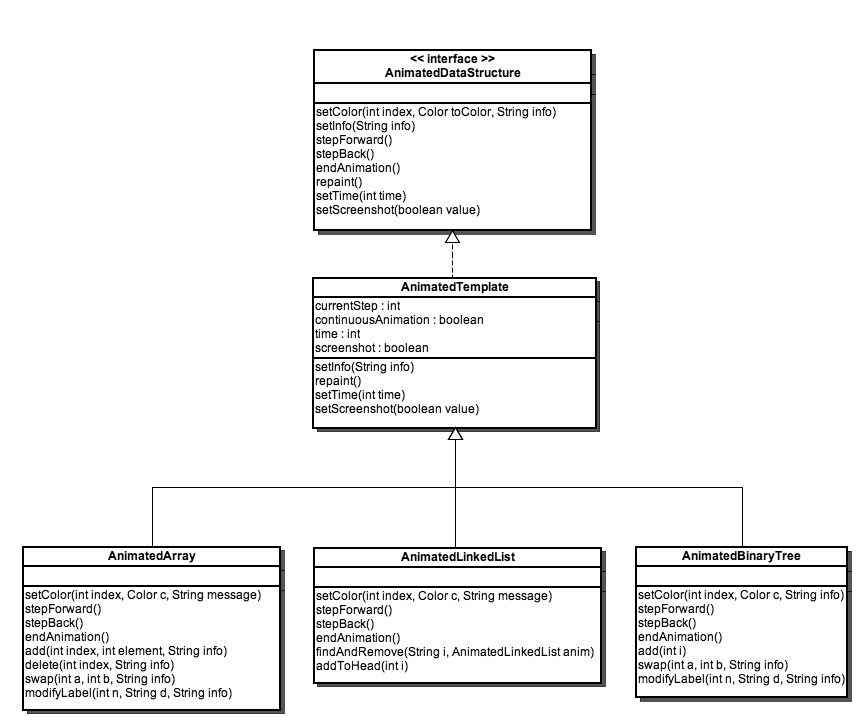
\includegraphics[width=\textwidth]{images/refactoring.png}
\end{center}
\caption{Structure after refactoring (does not include all methods and variables)}
\label{fig:refactoring}
\end{figure}

\subsection{Liam Bell}

%==============================================================================
\chapter{Evaluation}

TODO

%==============================================================================
\chapter{Conclusion}
To conclude, we feel that the experience of building our Algorithm Animator as a group has been incredibly interesting and engaging, but not without its challenges. The system we have built is able to produce a detailed visual animation for the algorithms that the user has built using our API. Our most successful development has been the step-based approach, which represents an animation as a series of steps, so that the user can step through each of their calls to our API as they are executed in turn, and watch them be successfully animated. Our implementation also allows the user to step back through their elapsed steps, should they require seeing part of the animation again.
We felt that the system could be generalised to a higher degree for the AnimatedArray class we built, given that there is a wider range of algorithms applicable to arrays. For instance, our system is able to accommodate numerous user constructed non-recursive sorting algorithms with our API. In contrast to this are the animated linked list and binary trees, which have operations that are restricted to their own data structures. However, our users will still be able to completely utilise their functionality with our data structure defined operations, and successfully animate them.

For future development, we would consider broadening our range of data structures in order for our users to exercise a wider range of algorithms that they desire to animate. With this approach, the user will gain a deeper understanding into their own programmed algorithms and the data structures which perform them.
Our system will also require some debugging to iron out issues and keep it fit for purpose. We believe these factors will increase the appreciation of our users, and serve as a more beneficial teaching tool for the visual analysis of algorithms.



%==============================================================================
\section{Contributions}
\subsection{Arthur Bigeard}
\subsection{Alexander Ferguson}
\subsection{Andrew Gibson}
\begin{itemize}
	\item Graphics framework research and justifying selection
	\item Initial framework implementation with animation
	\item AnimatedLinkedList built using existing step-by-step prototype
	\item Assisting other members with issues and proposing solutions
	\item Staying up to date with the repository; uploading changes
and checking its integrity.
\end{itemize}
\subsection{Gediminas Leikus}
\label{Gediminas:Con}
\begin{itemize}
	\item Project planning
	\item Steps in animations prototype
	\item Continuous and step-by-step animation prototypes
	\item AnimatedArray individual functions implementations
	\item AnimatedArray animated algorithms examples
	\item Managing the repository, reviewing changes or updates
	\item Refactoring
	\item Debugging issues encountered by other members and looking for solutions
	\item Sections or contributions to sections Abstract, \ref{intro}, \ref{PE:steps}, \ref{PE:refactoring} and \ref{Gediminas:Con} of this document
\end{itemize}
\subsection{Liam Bell}

%==============================================================================
\appendix

\chapter{Glossary}

Including expansions of non-standard abbreviations, acronyms and other key definitions.
\section{API}
Application Programming Interface - is a protocol intended to be used as an interface by software components to communicate with each other.

\chapter{Maintenance document}

TODO

summarization of the delivered software, identifying all major deficiencies

\chapter{User manual}

Our API consists of 3 data structure you can animate:
\begin{itemize}
\item Arrays
\item Heaps
\item LinkedLists
\end{itemize}

To begin with the API you are provided a simple Main class with a few lines of required code to run the animation.

\begin{figure}
\begin{center}
\begin{verbatim}


import java.awt.Color;

import AnimatedDataStructure.AnimatedDataStructure;
import AnimatedLinkedList.AnimatedLinkedList;
import AnimatedArray.AnimatedArray;

import java.util.Random;

public class Main {
    
    private static AnimatedDataStructure anim; //Declare the AnimatedDataStructure you want
	//to animate here
    public static int time = 200;
    
	public static void main(String[] args) {
        anim.endAnimation();
	}
	
}

\end{verbatim}
\end{center}
\caption{The Main class code}
\label{fig:main}
\end{figure}

The first thing you will need to do is instanciate an Animation object of the data structure you want to animate. There are two constructors for
each animated data structure from which you can choose:
\begin{itemize}
\item The default constructor which only requires you to pass an array of data
\item The custom window size constructor which takes 3 parameters: the array of data, the window width and window height
\end{itemize}

Each data structure has different animation calls which you can use to create your animation steps within your algorithm.
Every structure support the following calls:
\begin{itemize}
\item swap: takes the indexes of two elements to swap and a String to label the step
\item setColor: takes the index of the element changing color, a Color ENUM value and a String to label the step
\item setInfo: takes a parameter String to display as an animation information
\item setTime: takes a parameter Integer (expressing milliseconds) to set the speed of the next step created
\end{itemize}

The Array supports the following additional calls:
\begin{itemize}
\item add : takes 3 parameter: the index position to add the element to, the integer value of the element and a String to label the step
\item delete : removes the element at the Integer index i, and takes a String to label the step
\end{itemize}

The LinkedList supports the following additional calls:
\begin{itemize}
\item findAndRemove: Find and removes the elements equal to a String s in a parameter AnimatedLinkedList and a String to label the step
\item addToHead : adds the integer value i at the head of the LinkedList and a String to label the step
\end{itemize}

The Heap supports the following additional call:
\begin{itemize}
\item add : adds the integer value i to the heap; this function maintains the binary tree ordered structure. It also takes a second String parameter to label the step
\end{itemize}

To animate your algorithm you have to inject the appropriate API calls into your code where you manipulate your data structure, or when you want
do some highlighting on elements. Here is a sample animation code for an array sorting algorithm:

\begin{figure}
\begin{center}
\begin{verbatim}


import java.awt.Color;

import AnimatedDataStructure.AnimatedDataStructure;
import AnimatedLinkedList.AnimatedLinkedList;
import AnimatedArray.AnimatedArray;

import java.util.Random;

public class Main {
    
    private static AnimatedArray anim;//We're creating an animation on an array,
    //hence using the AnimatedArray AnimatedDataStructure
    public static int time = 200;

    public static void main(String[] args) {
        int[] arr = {1,2,3,4,5,6,7,8,9,0,1,2,3,4};
        anim = new AnimatedArray(arr);
        int i, j,t=0;
        for(i = 0; i < arr.length; i++){
            for(j = 1; j < (arr.length-i); j++){
                anim.setColor(j, Color.RED, "");
                anim.setColor(j-1, Color.RED, "");
                if(arr[j-1] > arr[j]){
                    t = arr[j-1];
                    arr[j-1]=arr[j];
                    arr[j]=t;
                    anim.swap(j, j-1, "Swapping");
                }
                anim.setColor(j, Color.BLUE, "");
                anim.setColor(j-1, Color.BLUE, "");
            }
            anim.setColor(j-1, Color.DARK_GRAY, "Gray out an element that's in it's place already.");
        }
        anim.endAnimation();
    }
	
}

\end{verbatim}
\end{center}
\caption{An array sorting algorithm example: bubblesort}
\label{fig:animationAlgorithm}
\end{figure}



\chapter{User interface}

The user interface is very simple and only consists in a few explicitely named button.

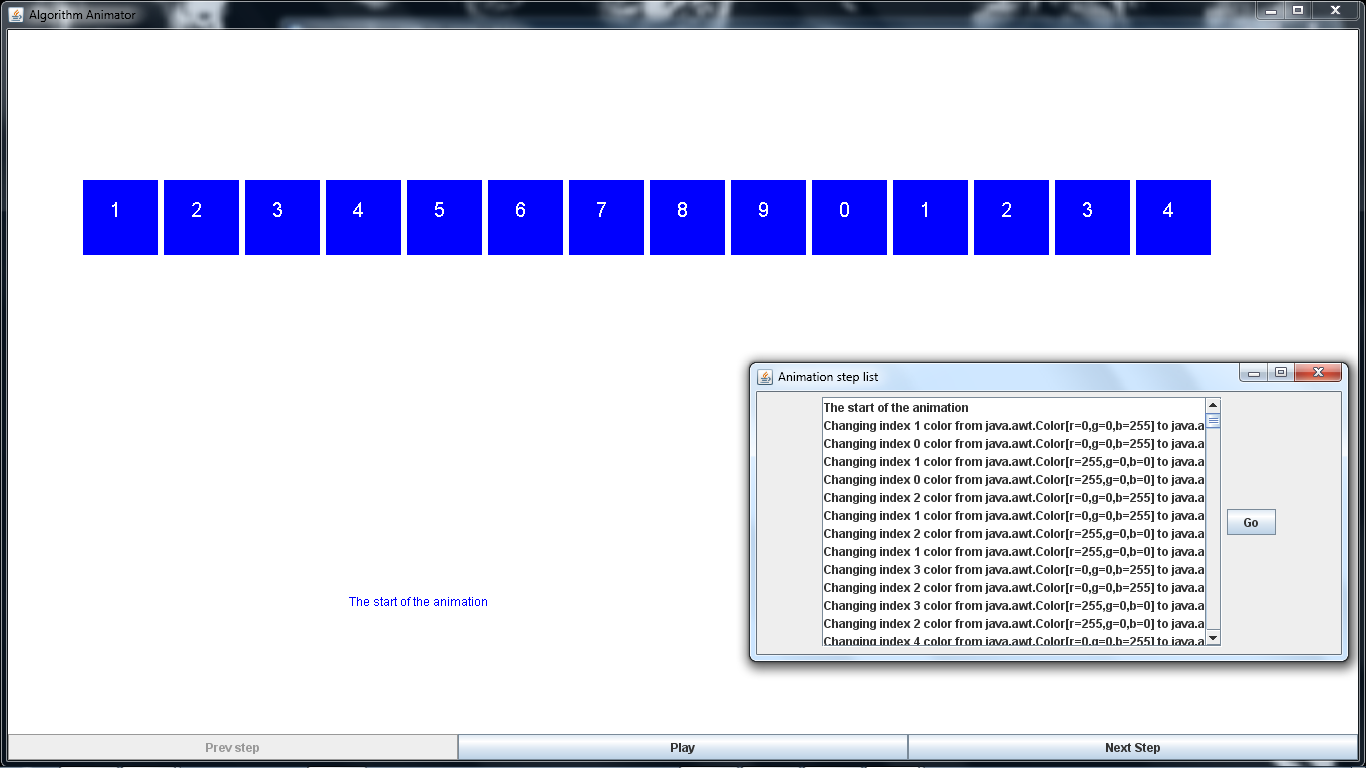
\includegraphics[width=\textwidth]{images/animationWindow.png}

When running the animation, you may use the middle Play/Pause button to run or stop the animation. There's two distinct animation
behaviours depending on wether the animation is running or not:
\begin{itemize}
\item If the animation is running, you won't be able to use the Prev/Next Step buttons
\item If the animation is paused, you may run it step by step using the Prev/Next Step buttons
\end{itemize}

Please take note that the Prev Step button will not animate the rollback to the previous step, it will simply restore the state of the animation to its previous state.
The Next Step Button on another hand will animate the change of state to the next step.

There is a second window opened with every animation running. It contains the entire list of animation steps, identified by their step description. When the animation is paused,
you may jump backward or forward in the animation by selecting the step you want to jump to and clicking the Go button. 
Please note that you may only use this feature while the animation is paused.

\bibliographystyle{plain}
\bibliography{example}
\end{document}
